% vim:autoindent:set textwidth=78:
\chapter{Working with Vector Data}
QGIS supports vector data in a number of formats, including shapefiles,
MapInfo mif, and PostGIS\index{PostGIS} layers in a PostgreSQL database. Support for
additional data types is provided by plugins, for example delimited
text\index{delimited text}.

This section describes how to work with two common formats:
shapefiles\index{shapefile} and PostGIS\index{PostGIS} layers. Many of the
features available in QGIS work the same regardless of the vector data source.
This is by design and includes the identify, select, labeling, and attributes
functions.

\section{Shapefiles}\index{shapefile}
Shapefile support is provided by a library of functions (OGR
\url{http://www.remotesensing.org/gdal/ogr})\index{ogr}. See Appendix
\ref{appdx_ogr} for a list of supported formats.

A shapefile actually consists of a minimum of three
files:\index{shapefile!format}
\begin{compactenum}
\item .shp file containing the feature geometries
\item .dbf file containing the attributes in dBase format
\item .shx index file
\end{compactenum}
The technical specification for the shapefile format can be found at\\
\url{http://www.esri.com/library/whitepapers/pdfs/shapefile.pdf}\index{shapefile!specification}.
\subsection{Loading a Shapefile}
\parpic[l]{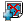
\includegraphics{qgis_user_guide_images/addshapefile}}To load a
shapefile, start QGIS and click on the \textit{Add a vector layer} toolbar bar
button\index{shapefile!loading}. This same tool can be used to load any of the formats supported by the OGR library.

Clicking on the tool brings up a standard open file dialog (Figure \ref{fig:openshapefile}) which allows you to navigate the file system and load a shapefile (or other supported data source). 
You can also select the Encoding type for the shapefile if desired.
\begin{figure}[h]
   \begin{center}
   \caption{Open OGR Data Source Dialog}\label{fig:openshapefile}\smallskip
   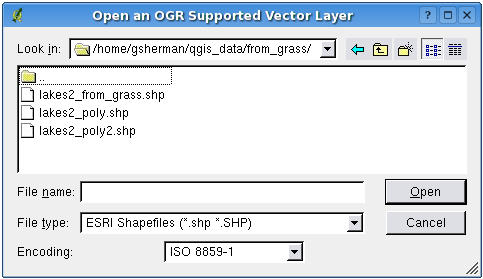
\includegraphics[scale=.75]{qgis_user_guide_images/shapefileopendialog}
\end{center}  
   
\end{figure}
Selecting a shapefile from the list and clicking Ok loads it into QGIS. Figure
\ref{fig:loadedshapefile} shows QGIS after loading the country.shp file.
\begin{figure}[h]
   \begin{center}
   \caption{QGIS with the countries Shapefile Loaded}\label{fig:loadedshapefile}\smallskip
   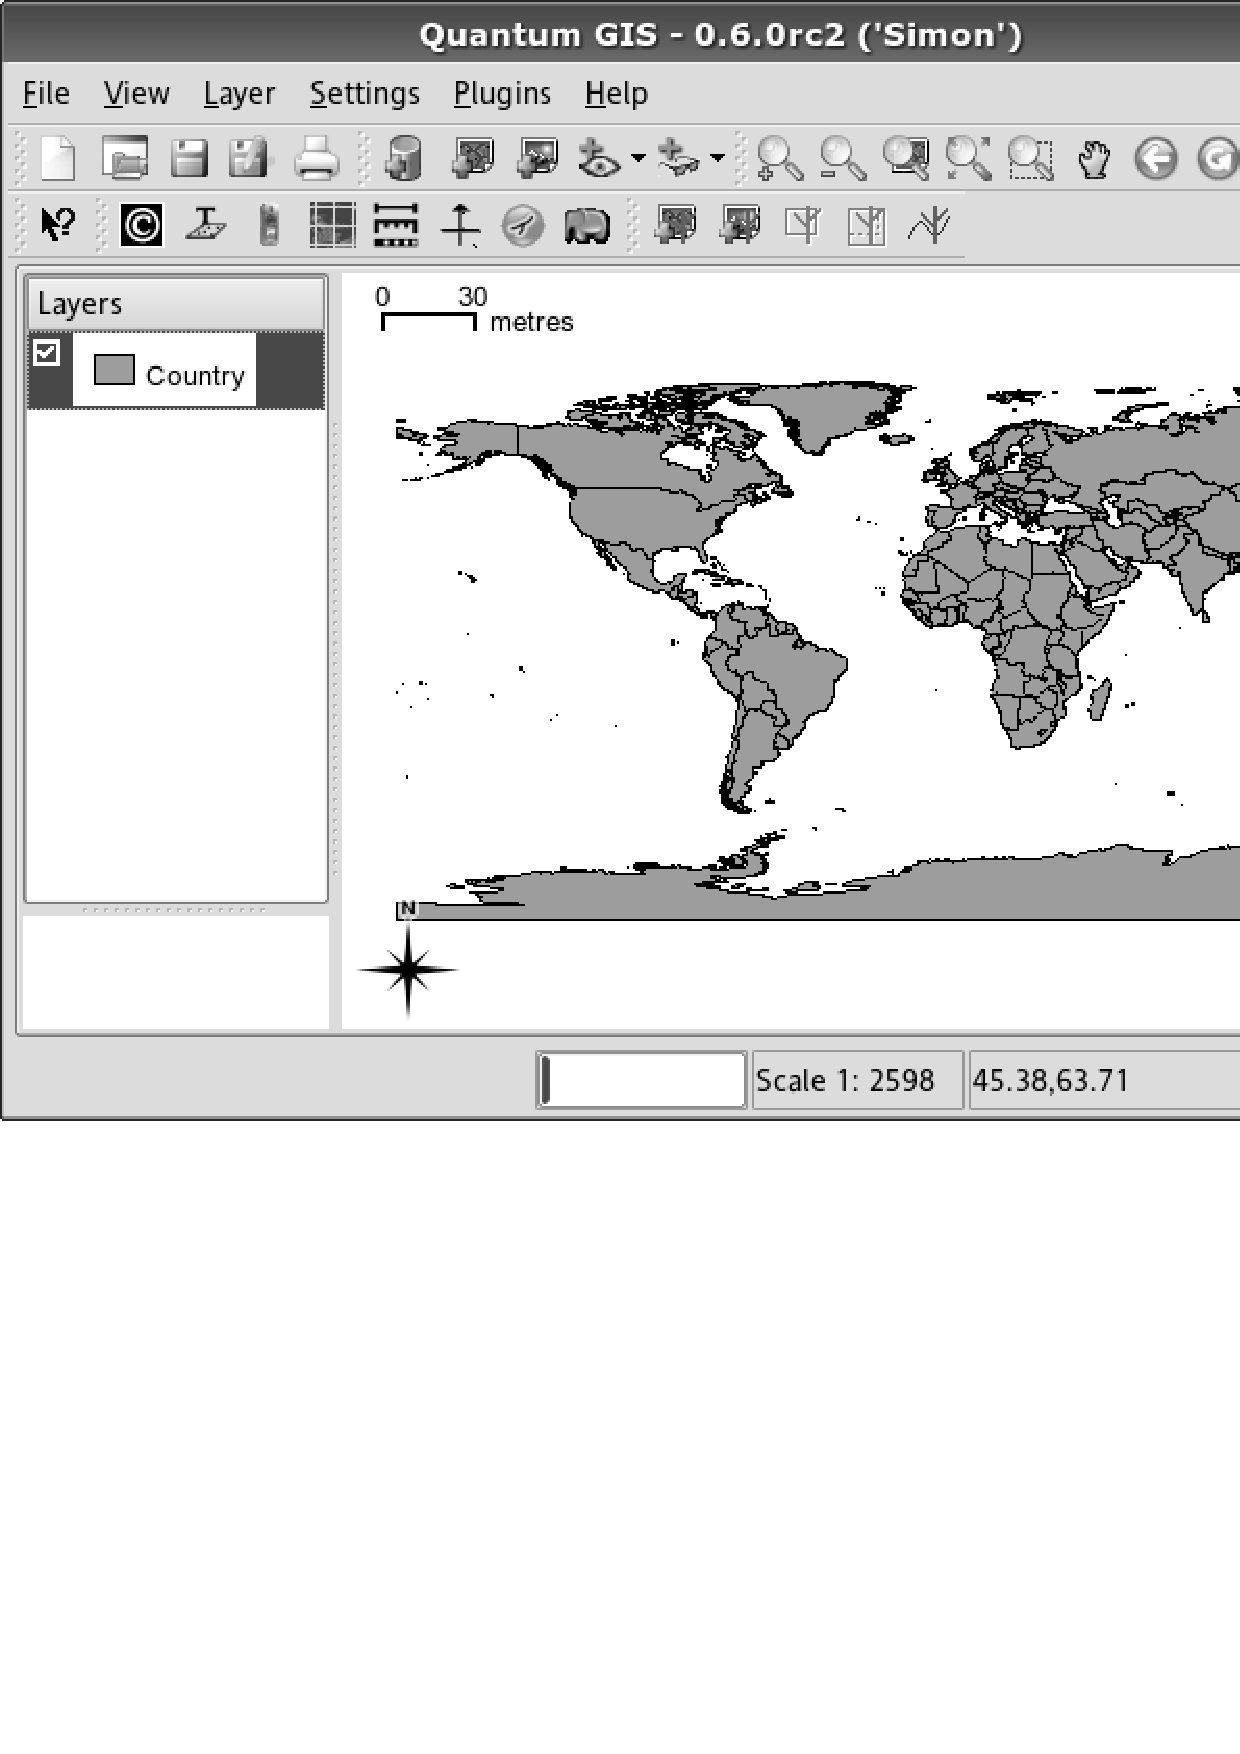
\includegraphics[scale=.7]{qgis_user_guide_images/shapefileloaded}
\end{center}  
   
\end{figure}
\begin{Tip}\caption{\textsc{Layer Colors}}
\qgistip{When you add a layer to the map, it is assigned a random color. When adding more than one layer at a time, different colors are assigned to each. }
\end{Tip}

Once loaded, you can zoom around the shapefile using the map navigation tools. To change the symbology of a layer, open the layer properties dialog by double clicking on the layer name or by right-clicking on the name in the legend and choosing \textsl{Properties} from the popup menu. See Section \ref{sec:symbology} for more information on setting symbology of vector layers.
\subsection{Loading a MapInfo Layer}
To load a MapInfo layer, click on the \textit{Add a vector layer}
toolbar bar button and change the file type filter to \textit{MapInfo (*.mif
*.tab *.MIF *.TAB)} and select the layer you want to load.

\subsection{Loading an ArcInfo Coverage}
Loading an an ArcInfo coverage is done using the same method as with a
shapefiles and MapInfo layers. Click on the \textit{Add a vector layer} toolbar
button to open the layer dialog.  Navigate to the coverage directory and select
one of the following files (if present in your coverage)
\begin{compactenum}
\item .lab - to load a label layer (polygon labels, or standing points
\item .cnt - to load a polygon centroid layer 
\item .arc - to load an arc (line) layer
\item .pal - to load a polygon layer
\end{compactenum}

\section{PostGIS Layers}\index{PostGIS!layers}
PostGIS layers are stored in a PostgreSQL database. The advantage of PostGIS is the spatial indexing, filtering, and query capability. Using PostGIS, vector functions such as select and identify work more accurately than with OGR layers in QGIS.
To use PostGIS layers you must:\index{PostgreSQL!loading layers}
\begin{compactenum}
\item Create a stored connection in QGIS to the PostgreSQL database (if one is
not already defined)\index{PostgreSQL!connection}
\item Connect to the database
\item Select the layer to add to the map
\item Optionally provide a SQL \textit{where} clause to define which features to load from the layer
\item Load the layer
\end{compactenum}
\subsection{Creating a Stored Connection}\index{PostgreSQL!connection}
\parpic[l]{
\includegraphics{qgis_user_guide_images/addpostgis}}The first time
you use a PostGIS data source, you must create a connection to the PostgreSQL
database that contains the data. Begin by clicking on the \textit{Add a PostGIS
Layer} toolbar button. The \textsl{Add PostGIS Table(s)} dialog will be
displayed. To access the connection manager\index{PostgreSQL!connection
manager}, click on the \textsl{New} button to
display the \textsl{Create a New PostGIS Connection} dialog. The parameters
required for a connection are shown in Table \ref{tab:postgis_connection_parms}.
\begin{table}[h]\index{PostgreSQL!connection parameters}
\centering
\caption{PostGIS Connection Parameters}\label{tab:postgis_connection_parms}\medskip
 \begin{tabular}{|l|p{5in}|}
\hline Name & A name for this connection. Can be the same as \textsl{Database}
\\
\hline Host \index{PostgreSQL!host}
& Name of the database host. This must be a resolvable host name the same as would be used to open a telnet connection or ping the host \\
\hline Database \index{PostgreSQL!database} & Name of the database  \\
\hline Port \index{PostgreSQL!port}& Port number the PostgreSQL database server listens on. The default port is 5432.\\
\hline Username \index{PostgreSQL!username}& User name used to login to the database \\
\hline Password \index{PostgreSQL!password}& password used with \textsl{Username} to connect to the database\\
\hline
\end{tabular}
\end{table}
Once the parameters have been filled in, you can test the connection by clicking
on the \textsl{Test Connection} button\index{PostgreSQL!connection!testing}. To save the password with the connection information, check the \textsl{Save Password} option.
\begin{Tip}\caption{\textsc{QGIS User Settings and
Security}}\index{settings}\index{security}
\qgistip{Your customized settings for QGIS are stored based on the operating system. On Linux/Unix, the settings are stored in your home directory in .qt/qgisrc. On Windows, the settings are stored in the registry. Depending on your computing environment, storing passwords in your QGIS settings may be a security risk.
}
\end{Tip}
\subsection{Loading a PostGIS Layer}\index{PostgreSQL!loading layers}
\parpic[l]{
\includegraphics{qgis_user_guide_images/addpostgis}}Once you have one or more connections defined, you can load layers from the PostgreSQL database. Of course this requires having data in PostgreSQL. See Section \ref{sec:loading_postgis_data} for a discussion on importing data into the database. 

To load a layer from PostGIS, perform the following steps:
\begin{compactenum}
\item If the PostGIS layer dialog is not already open, click on the \textit{Add a PostGIS Layer} toolbar button
\item Choose the connection from the drop-down list and click \textsl{Connect}
\item Find the layer you wish to add in the list of available layers
\item Select it by clicking on it. You can select multiple layers by holding down the shift key while clicking. See Section \ref{sec:query_builder} for information on using the PostgreSQL Query Builder to further define the layer.
\item Click on the \textsl{Add} button to add the layer to the map
\end{compactenum}
\begin{Tip}\caption{\textsc{PostGIS Layers}}
\qgistip{Normally a PostGIS layer is defined by an entry in the geometry\_columns table. At version 0.7, QGIS can load layers that do not have an entry in the geometry\_columns table. This includes both tables and views. Defining a spatial view provides a powerful means to visualize your data.}
\end{Tip}
\subsection{Using the Query
Builder}\label{sec:query_builder}\index{PostgreSQL!query builder}
The PostgreSQL Query Builder allows you to define a subset of a table and add it
as a layer in QGIS.  For example, if you have a towns layer with a population
field you could select only larger towns by entering \textsl{population >
100000} in the SQL box of the query builder. Figure \ref{fig:querybuilder} shows an
example of the query builder populated with data from a layer in PostgreSQL. 

\begin{figure}[h]
  \begin{center}
    \caption{PostgreSQL Query Builder}\label{fig:query_builder}\smallskip
    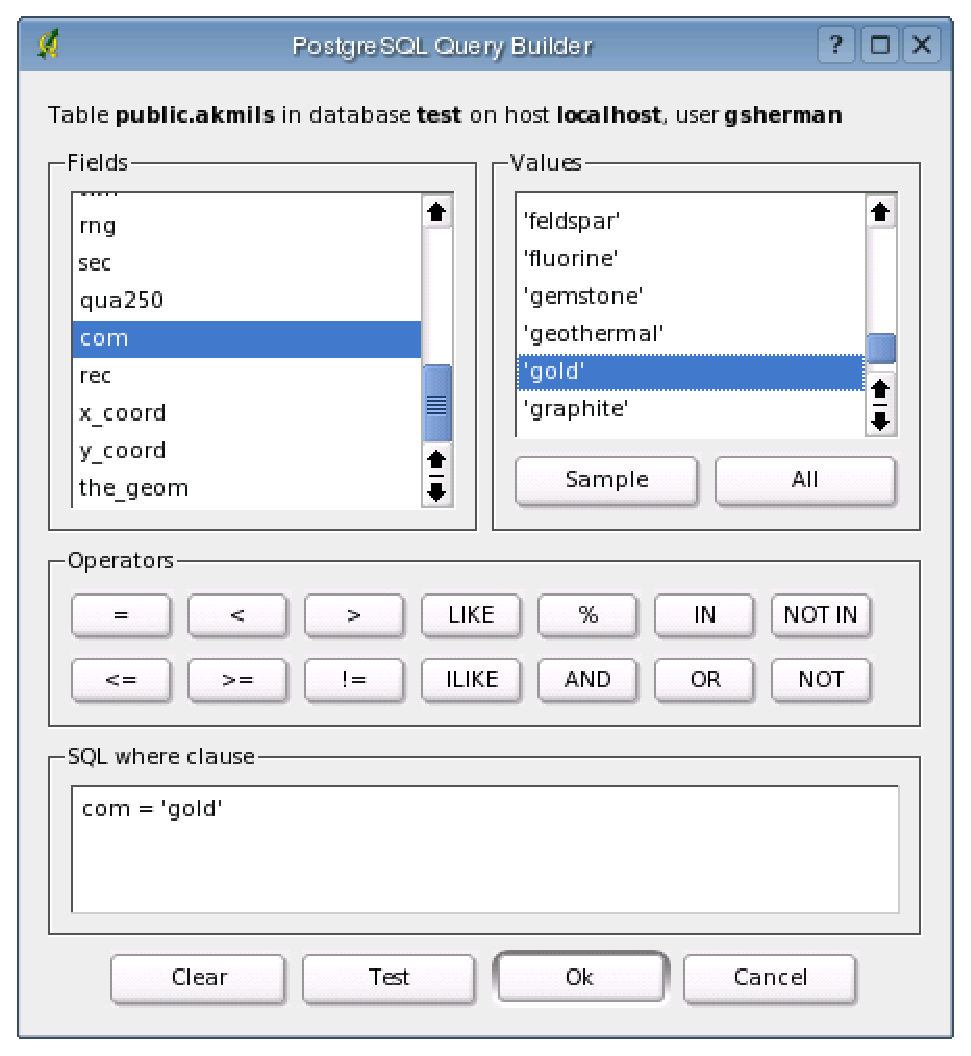
\includegraphics[scale=.6]{qgis_user_guide_images/querybuilder}
  \end{center}  
\end{figure}

The query builder\index{query builder} lists the layer's database
fields in the list box on the left.  You can get a sample of the data contained
in the highlighted field by clicking on the \textit{Sample} button\index{query
builder!generating sample list}. This
retrieves the first 25 distinct values for the field from the database. To get a
list of all possible values for a field, click on the \textit{All}
button\index{query builder!getting all values}. To
add a selected field or value to the query, double-click on it\index{query
builder!adding fields}. You can use the
various buttons to construct the query or you can just type it into the SQL box.

To test a query, click on the \textit{Test} button\index{query builder!testing
queries}. This will return a count of
the number of records that will be included in the layer. When satisfied with
the query, click \textit{Ok}. The SQL for the where clause will be shown in the
SQL column of the layer list.


\begin{Tip}\caption{\textsc{Changing the Layer Definition}}\index{query
builder!changing layer definitions}
\qgistip{You can change the layer definition after it is loaded by altering the
SQL query used to define the layer. To do this, open the vector layer properties
dialog by double-clicking on the layer in the legend and click on the
\textit{Query Builder} button on the \textit{General} tab. See Section
\ref{sec:vectorprops} for more information.}
\end{Tip}

\subsection{Some details about PostgreSQL layers}\label{sec:postgis_details}
\index{PostgreSQL!layer details}
This section contains some details on how QGIS accesses PostgreSQL
layers. Most of the time QGIS should simply provide you with a list of
database tables that can be loaded, and load them on request. However,
if you have trouble 
loading a PostgreSQL table into QGIS, the information below may help
you understand any QGIS messages and give you direction on changing
the PostgreSQL table or view definition to allow QGIS to load it.

QGIS requires that PostgreSQL layers contain a column that can be
used as a unique key for the layer. For tables this usually means
that the table needs a primary key, or have a column with a unique
constraint on it. QGIS additionally requires that this column be of
type int4 (an integer of size 4 bytes). If a table lacks these items,
the oid column will 
be used instead. Performance will be improved if the column is
indexed (note than primary keys are automatically indexed in PostgreSQL). 

If the PostgreSQL layer is a view the same requirements exist, but
views don't have primary keys or columns with unique constraints on
them. In this case QGIS will try to find a column in the view that is
derived from a table column that is suitable. If one cannot be found,
QGIS will not load the layer. If this occurs, the solution is to alter
the view so that it does include a suitable column (a type of int4
and either a primary key or with a unique constraint, preferably indexed).

\subsection{Importing Data into PostgreSQL}\label{sec:loading_postgis_data}
\index{SPIT!importing data}
Data can be imported into PostgreSQL using a number of methods. PostGIS
includes a utility called shp2pgsql that can be used to import shapefiles into
a PostGIS enabled database. For example, to import a shapefile named lakes into a PostgreSQL database named gis\_data, use the following command:
\begin{verbatim} 
  shp2pgsql -s 2964 lakes.shp lakes_new | psql gis_data
\end{verbatim}
This creates a new layer named lakes\_new in the the gis\_data database. The new layer will have a spatial reference identifier (SRID) of 2964. See Section \ref{sec:projections} for more information on spatial reference systems and projections.

\parpic[l]{
\includegraphics{qgis_user_guide_images/spiticon}}QGIS comes with a
plugin named SPIT (Shapefile to PostGIS Import Tool)\index{SPIT}.
SPIT can be used to load multiple shapefiles at one time and includes support
for schemas. To use SPIT, open the Plugin Manager from the Tools menu and load
the plugin by checking the box next to the SPIT plugin and click Ok. The SPIT
icon will be added to the plugin toolbar\index{SPIT!loading}. 

To import a shapefile, click on the SPIT tool in the toolbar to open the dialog.
You can add one or more files to the queue by clicking on the \textsl{Add}
button. To process the files, click on the Import button. The progress of the
import as well as any errors/warnings will be displayed as each shapefile is
processed.  
\begin{Tip}\caption{\textsc{Importing Shapefiles Containing
PostgreSQL Reserved Words}}\index{SPIT!reserved words}
\qgistip{If a shapefile is added to the queue containing fields that are
reserved words in the PostgreSQL database a dialog will popup showing the status
of each field. You can edit the field names\index{SPIT!editing field names}
prior to import and change any that are reserved words (or change any other
field names as desired). Attempting to
import a shapefile with reserved words as field names will likely fail.}
\end{Tip} 
\section{The Vector Properties
Dialog}\label{sec:vectorprops}\index{vector layers!properties dialog} The
vector properties dialog provides information about a layer, symbology
settings, and labeling options. If your vector layer has been loaded from a
PostgreSQL / PostGIS datastore, you can also alter the underlying SQL for the
layer - either by hand editing the SQL on the \textit{General} tab, or by
invoking the query builder dialog on the \textit{General} tab. To access the
properties dialog, double-click on a layer in the legend or right-click on the
layer and select Properties from the popup menu.

\subsection{Vector Symbology}\label{sec:symbology}\index{vector
layers!symbology}

QGIS supports a number of symbology renderers to control how
vector features are displayed. Currently the following renderers
are available:

\begin{compactdesc}
    \item[Single symbol] - a single style is applied to every
    object in the layer.\index{vector layers!renderers!single symbol}
    \item[Graduated symbol] - objects within the layer are
    displayed with different symbols classified by the values of a
    particular field.\index{vector layers!renderers!graduated symbol}
    \item[Continuous colour] - objects within the layer are
    displayed with a spread of colours classified by the numerical
    values within a specified field.\index{vector layers!renderers!continuous color}
    \item[Unique value] - objects are classified by the unique
    values within a specified field with each value having a
    different symbol.\index{vector layers!renderers!unique value}
\end{compactdesc}

For layers containing point features, additional renderers are
available that use SVG icons:

\begin{compactdesc}
    \item[Single marker] - a single specified icon is used for
    every point within the layer.\index{vector layers!renderers!single marker}
    \item[Graduated marker] - points within the layer are
    displayed with different icons classified by values within a
    particular field.\index{vector layers!renderers!graduated marker}
    \item[Unique value marker] - points are classified by unique
    values within a specified field with each value having a
    different icon.\index{vector layers!renderers!unique value marker}
\end{compactdesc}

To change the symbology for a layer, simply double click on its legend entry and
the vector layer properties dialog will be shown.\index{symbology!changing}

\begin{figure}[h]
   \begin{center}
   \caption{Vector Layer Properties Dialog}\label{fig:vector_symbology}\smallskip
   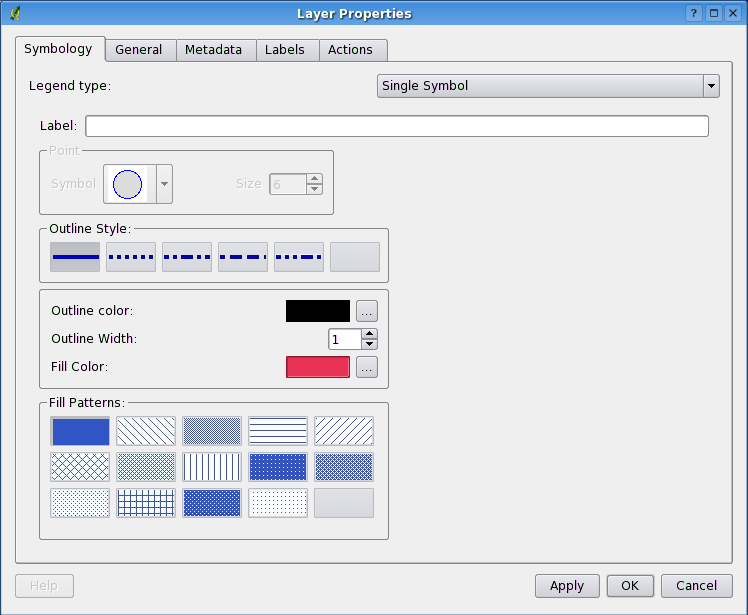
\includegraphics[scale=.5]{qgis_user_guide_images/vectorLayerSymbology}  
\end{center}  
\end{figure}
%force all figures to be printed
\section{Attribute Actions}\index{actions}
QGIS provides the ability to perform an action based on the attributes of a
feature. This can be used to perform any number of actions, for example,
running a program with arguments built from the attributes of a feature or
passing parameters to a web reporting tool.

Actions are useful when you frequently want to run an external application or
view a web page based on one or more values in your vector layer. An example is
performing a search based on an attribute value. This concept is used in the
following discussion.

\subsection{Defining Actions}\index{actions!defining}
Attribute actions are defined from the vector layer properties dialog. To define
an action, open the vector layer properties dialog and click on the
\textit{Actions} tab. Provide a descriptive name for the action. The action
itself must contain the name of the application that will be executed when the
action is invoked. You can add one or more attribute field values as arguments
to the application. When the action is invoked any set of characters that start
with a \% followed by the name of a field will be replaced by the value of that
field.  The special characters \%\% \index{\%\%}will be replaced by the value of
the field that was selected from the identify results or attribute table (see
Using Actions below).  Double quote marks can be used to group text into a
single argument to the program, script or command. Double quotes will be ignored
if proceeded by a backslash.  

Two example actions are shown below:\index{actions!examples}
\begin{compactenum}
  \item \texttt{konqueror http://www.google.com/search?q=\%nam}
  \item \texttt{konqueror http://www.google.com/search?q=\%\%}
\end{compactenum}
In the first example, the web browser konqueror is invoked and passed a URL to
open. The URL performs a Google search on the value of the \textit{nam} field
from our vector layer. Note that the application or script called by the action
must be in the path or you must provided the full path. To be sure, we could
rewrite the first example as: \texttt{/opt/kde3/bin/konqueror
http://www.google.com/search?q=\%nam}. This will ensure that the konqueror
application will be executed when the action is invoked.

The second example uses the \%\% notation which does not rely on a particular
field for its value. When the action is invoked, the \%\% will be replaced by
the value of the selected field in the identify results or attribute table.

\subsection{Using Actions}\index{actions!using}
Actions can be invoked from either the \textit{Identify Results} dialog or the
\textit{Attribute table} dialog. To invoke an action, right click on the record
and choose the action from the popup menu. Actions are listed in the popup menu
by the name you assigned when defining the actions. Click on the action you wish
to invoke.

If you are invoking an action that uses the \%\% notation, right-click on the
field value in the \textit{Identify Results} dialog or the
\textit{Attribute table} that you wish to pass to the application or script.

Here is another example that pulls data out of a vector layer and inserts it
into a file using bash and the `echo' command (so it will only work on Gnu/Linux
and perhaps Mac OS X). The layer in question has fields for a species name
(taxon\_name), latitude (lat) and longitude (long). I would like to be able to
make a spatial selection of a localities and export these field values to a text
file for the selected record (shown in yellow in the QGIS map area). Here is the
action to achieve this:

\begin{verbatim}
	bash -c "echo \"%taxon_name %lat %long\" >> /tmp/species_localities.txt"
\end{verbatim} 

After selecting a few localities and running the action on each one, opening the output file will show something like this:

\begin{verbatim}
	Acacia mearnsii -34.0800000000 150.0800000000
	Acacia mearnsii -34.9000000000 150.1200000000
	Acacia mearnsii -35.2200000000 149.9300000000
	Acacia mearnsii -32.2700000000 150.4100000000
\end{verbatim} 


\section{Editing}\index{editing}

QGIS supports basic capabilities for editing spatial data.  Before reading any
further you should note that at this stage editing support is still preliminary.
Before performing any edits, always make a backup of the dataset you are about
to edit. 

\textbf{Note} - the procedure for editing GRASS layers is different - see
Section \ref{grass_digitising} for details.

\subsection{Editing an Existing Layer}\index{editing!an existing layer}
\label{sec:edit_existing_layer}
If you wish to edit an existing layer, choose \textit{Start Editing} from the
context menu after right clicking on the legend entry for that layer. Remember
to backup your data before starting! Once the layer is in edit mode you will
see a small 
\includegraphics[scale=1]{qgis_user_guide_images/editable} icon to
remind you.\index{editing!icon}

Now that the layer is editable, you can use the \textit{Capture Points} icon (or
similar icon for line and polygon layers) on the toolbar to put the QGIS cursor
into digitising mode. If you are capturing a point feature simply use the pan
and zoom tools to navigate to the area of interest, then click the
\textit{Capture Points} tool and click on the map area to create the  
new point feature. A window will appear allowing you to set the attributes.
Figure \ref{fig:vector_digitising} shows setting attributes for a fictitious
new city in the Antarctic.

\begin{figure}[h]
   \begin{center}
   \caption{Vector Digitizing Attributes Capture Dialog}\label{fig:vector_digitising}\smallskip
   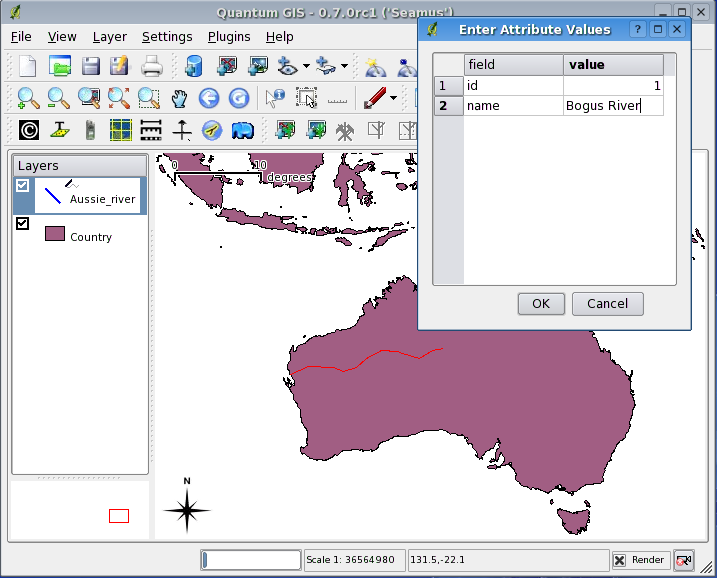
\includegraphics[scale=.65]{qgis_user_guide_images/digitising_attributes}
\end{center}  
\end{figure}

In its current implementation the attributes dialog box does not check that the
data matches the type expected, so make sure of this before
pressing \textit{Ok}. 

To delete a feature, select it using the selection tool and choose
\textit{Delete selection} from the editing tools.

Once you have finished adding features, choose \textit{Stop Editing} from the
layer's context menu. Choosing \textit{Yes} will save the changes to disk, while
choosing \textit{No} at this point will cause them to be discarded.
\index{editing!saving changes}
%Note that QGIS does not yet provide any way to delete an individual feature.

\subsection{Creating a New Layer}\index{editing!creating a new layer}

To create a new layer for editing, choose \textit{New Vector Layer} from the
\textit{Layer} menu. The \textit{New Vector Layer} dialog will be displayed as
shown in Figure \ref{fig:newvectorlayer}. Choose the type of layer (point,
line, or polygon). 
\begin{figure}[h]
   \begin{center}
   \caption{Creating a New Vector Dialog}\label{fig:newvectorlayer}\smallskip
   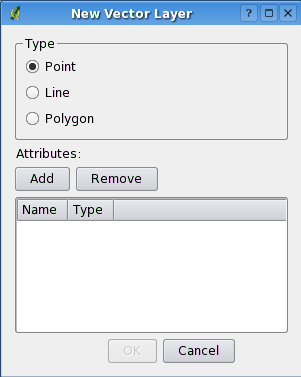
\includegraphics[scale=.75]{qgis_user_guide_images/newvectorlayer}
\end{center}  
Note that QGIS does not yet support creation of 2.5D
features (i.e. features with X,Y,Z coordinates) or measure features. At this
time, only shapefiles can be created. In a future version of QGIS, creation of
any OGR or PostgreSQL layer type will be supported.

\end{figure}
To complete the creation of the new layer, add the desired attributes by
clicking on the \textit{Add} button and specifying a name and type for the
attribute. Only real, integer, and string attributes are supported. Once you
are happy with the attributes, click Ok and provide a name for the shapefile.
QGIS will automatically add a .shp extension to the name you specify.  Once
the layer has been created, it will be added to the map and you can edit it in
the same way as described in Section \ref{sec:edit_existing_layer} above. 
